\section{Part II: the memory advantage is mostly a clock}
\label{sec:part2}

\subsection{The arms on the sealed panel}
\label{sec:part2-arms}

\Cref{tab:arms} and \cref{fig:part2-arms} give the confirmatory score of every arm. The LSTM
succeeds on 95.0\% of the sealed episodes. A memory-free MLP of the same size that is told the
time, MLP-wide + clock, reaches 91.7\%, and like the LSTM it acquires the task on every seed. The
same network without the clock falls to 65.1\%, close to the small MLP (61.9\%) and to the LSTM
whose memory is erased at every step (67.0\%). stack4 + clock is in between (74.2\%), with a wide
spread across seeds. \Cref{fig:part2-curves} shows that MLP-wide + clock even learns faster than
the LSTM during the first half of training, and that the three arms without a way to tell time
level off together around 55--60\% validation success.

\begin{table}[t]
  \centering
  \caption{Part II arms. Sealed: success of the validation-selected checkpoint on 64 new maps
  $\times$ 4 sampling seeds, mean over seeds with a 95\% bootstrap interval. Acquired: seeds
  meeting the acquisition rule within 300,000 interactions, with the median step among them.
  AUC: normalised area under the validation curve.}
  \label{tab:arms}
  \small
  \begin{tabular}{lrcccccc}
    \toprule
    Arm & Params & Clock & lr & Seeds & Sealed (\%) & Acquired & AUC \\
    \midrule
    LSTM & 11,367 & no & $10^{-3}$ & 20 & 95.0 [93.7, 96.3] & 20/20 (175k) & 0.60 \\
    MLP-wide + clock & 11,399 & yes & $10^{-3}$ & 20 & 91.7 [89.7, 93.5] & 20/20 (180k) & 0.62 \\
    stack4 + clock & 11,381 & yes & $3\cdot10^{-4}$ & 10 & 74.2 [69.3, 78.5] & 5/10 (270k) & 0.38 \\
    LSTM-reset & 11,367 & no & $10^{-3}$ & 20 & 67.0 [65.1, 68.8] & 2/20 (240k) & 0.45 \\
    MLP-wide, no clock$^\dagger$ & 11,401 & no & $10^{-3}$ & 10 & 65.1 [62.6, 67.6] & 0/10 & 0.44 \\
    MLP (small) & 2,919 & no & $10^{-3}$ & 10 & 61.9 [59.1, 64.6] & 0/10 & 0.46 \\
    \midrule
    LSTM-reset + clock$^\ddagger$ & 11,495 & yes & $10^{-3}$ & 10 & 91.5 [89.3, 93.4] & 10/10 (120k) & 0.68 \\
    MLP (small) + clock$^\ddagger$ & 2,951 & yes & $10^{-3}$ & 10 & 90.7 [88.4, 92.8] & 10/10 (205k) & 0.60 \\
    \bottomrule
    \multicolumn{8}{l}{\footnotesize $^\dagger$Added after an interim look; exploratory.
    $^\ddagger$Added after the confirmatory result; exploratory.}
  \end{tabular}
\end{table}

\begin{figure}[t]
  \centering
  \begin{minipage}[t]{0.49\linewidth}
    \centering
    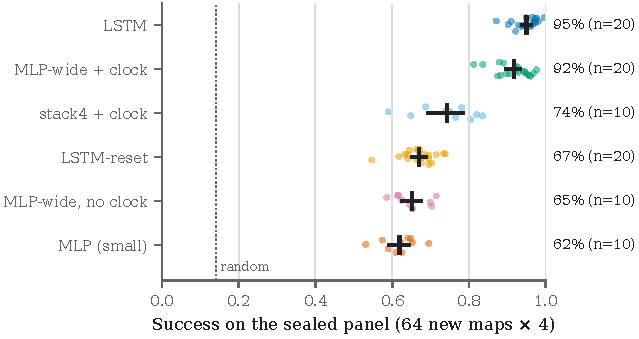
\includegraphics[width=\linewidth]{figures/fig_part2_arms.pdf}
    \caption{Sealed-panel success of every seed (dots), with the mean and its 95\% bootstrap
    interval (black).}
    \label{fig:part2-arms}
  \end{minipage}\hfill
  \begin{minipage}[t]{0.49\linewidth}
    \centering
    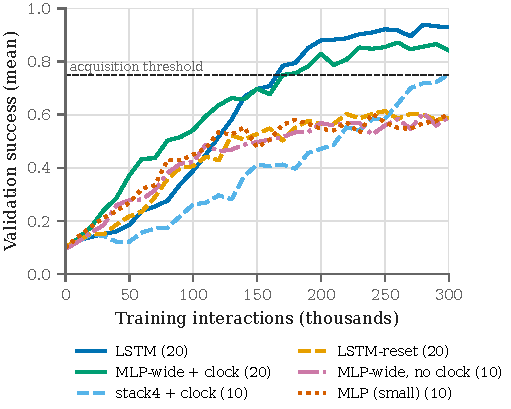
\includegraphics[width=\linewidth]{figures/fig_part2_curves.pdf}
    \caption{Mean validation success during training (number of seeds in brackets).}
    \label{fig:part2-curves}
  \end{minipage}
\end{figure}

\subsection{Confirmatory contrasts}
\label{sec:part2-contrasts}

\Cref{tab:contrasts} gives the preregistered contrasts on the sealed panel.

\textbf{P1 is not supported.} The LSTM is ahead of MLP-wide + clock by only 3.3\pp{}
$[0.9, 6.0]$, on 12 of 20 seeds. The difference is unlikely to be zero (Holm-adjusted
$p=0.041$), but it is far below the 15\pp{} the design required, and the AUC goes the other way
(on the development panel, $-2.8$\pp{} $[-4.6, -0.4]$). The 25 to 34\pp{} advantage of the LSTM
over the small MLP in the pilot and in Part~I is therefore not, for the most part, an advantage of
memory.

\textbf{P2 is supported.} Erasing the LSTM's state at every step costs 28.0\pp{} $[25.3, 29.9]$,
on all 20 seeds: the LSTM's advantage does depend on carrying a state from one step to the next.

\textbf{H3 is supported.} stack4 + clock stays well below the average of the LSTM and
MLP-wide + clock; it is even 17.5\pp{} below MLP-wide + clock, which has the same clock but no
stacked frames.

P1 and P2 together say that the LSTM needs its recurrent state, but that a network with no
memory at all does almost as well if it is told the time. The exploratory contrasts locate the
difference. Adding the clock to the wide MLP adds 26.6\pp{} $[21.5, 30.5]$ on all 10 shared
seeds; adding width without the clock adds 3.2\pp{} $[-0.4, 5.8]$, an interval that includes
zero. \Cref{fig:part2-ladder} adds the ingredients one at a time on the 10 seeds every arm shares:
of the 34\pp{} between the small MLP and the LSTM, width accounts for 9\%, the clock for 78\% and
what the LSTM does beyond a clock for 13\%.

The development panel gives the same verdicts (P1 $+4.9$\pp{} $[2.3, 8.0]$, not supported;
P2 $+32.1$\pp; H3 supported), so the conclusion does not depend on which panel or checkpoint is
used.

\begin{table}[t]
  \centering
  \caption{Contrasts on the sealed panel (percentage points). $p$: exact two-sided sign-flip
  test; Holm: adjusted within the family ($m=3$ principal, $m=5$ secondary). Ahead: seeds on
  which the contrast is positive. The exploratory family has no correction and no verdict.}
  \label{tab:contrasts}
  \small
  \begin{tabular}{llrcrrrc}
    \toprule
    & Contrast & Mean & BCa 95\% & $p$ & Holm & Ahead & Verdict \\
    \midrule
    P1 & LSTM $-$ MLP-wide + clock & $+3.3$ & [0.9, 6.0] & 0.021 & 0.041 & 12/20 & not supported$^*$ \\
    P2 & LSTM $-$ LSTM-reset & $+28.0$ & [25.3, 29.9] & $2\cdot10^{-6}$ & $6\cdot10^{-6}$ & 20/20 & supported \\
    H3 & LSTM $+$ MLP-wide $-$ 2 stack4 & $+39.2$ & [32.5, 47.9] & 0.002 & 0.010 & 10/10 & supported \\
    \midrule
    E1 & clock: MLP-wide $\pm$ clock & $+26.6$ & [21.5, 30.5] & 0.002 & & 10/10 & \\
    E2 & width: MLP-wide, no clock $-$ MLP & $+3.2$ & [$-0.4$, 5.8] & 0.092 & & 9/10 & \\
    E3 & LSTM $-$ MLP (small) & $+34.1$ & [31.6, 38.2] & 0.002 & & 10/10 & \\
    E4 & LSTM $-$ stack4 & $+21.8$ & [17.8, 27.4] & 0.002 & & 10/10 & \\
    E5 & stack4 $-$ MLP-wide + clock & $-17.5$ & [$-21.0$, $-13.6$] & 0.002 & & 0/10 & \\
    E6 & LSTM-reset $-$ MLP (small) & $+5.5$ & [2.1, 9.2] & 0.018 & & 8/10 & \\
    \bottomrule
    \multicolumn{8}{l}{\footnotesize $^*$Holm $p<0.05$ and interval above 0, but the mean is
    below the 15\,pp threshold.}
  \end{tabular}
\end{table}

\begin{figure}[t]
  \centering
  \begin{minipage}[c]{0.52\linewidth}
    \centering
    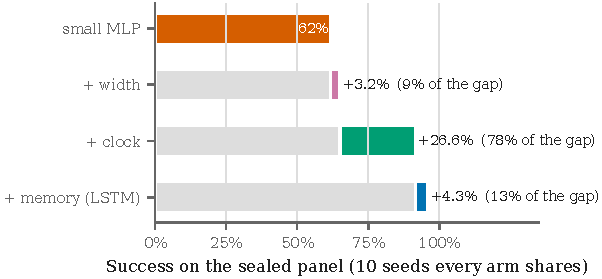
\includegraphics[width=\linewidth]{figures/fig_part2_ladder.pdf}
  \end{minipage}\hfill
  \begin{minipage}[c]{0.44\linewidth}
    \caption{From the small MLP to the LSTM, one ingredient at a time, on the 10 seeds that every
    arm shares (sealed panel). Width alone adds little; telling a memory-free network the time
    closes most of the gap.}
    \label{fig:part2-ladder}
  \end{minipage}
\end{figure}

\subsection{Why a clock?}
\label{sec:part2-why}

The task suggests a reason. Episodes are cut at 32 steps and the
success reward, $1-0.9\,t/32$, falls with time, so the value of a state depends on how many steps
are left. A critic that cannot tell time sees the same observation early and late in an episode
and must average two different values, which degrades the advantage estimates that drive A2C's
policy update; this is the failure mode \citet{pardo2018timelimits} describe. An LSTM can count
steps in its state, and LSTM-reset cannot, which would explain why P2 is large while P1 is small.

\paragraph{The LSTM's state encodes the time step.}
A linear probe reads the step $t$ from the trained LSTM's state with an out-of-fold $R^2$ of 0.84
(mean over 20 seeds; \cref{tab:probe}). Some of this is free: at its initial weights the same
network already reaches 0.52, because a recurrent state drifts as it integrates inputs. Training
increases it on 19 of 20 seeds. The observation alone carries no usable information about $t$
($R^2<0$), nor does LSTM-reset, whose state is erased at every step. The LSTM therefore has, and
learns to sharpen, exactly the information the clock gives the memory-free arms.

\paragraph{The time step alone closes the gap, whatever the network.}
A probe shows that the information is there, not that it matters. The two mechanism arms test
that directly (\cref{tab:arms,tab:mechanism}). Giving the clock to LSTM-reset, the network whose
memory is erased at every step, raises it from 67.0\% to 91.5\% (+24.1\pp{} $[21.6, 27.0]$ on all
10 seeds): of the 28 points the LSTM loses when its state is erased, the clock alone gives back
24. LSTM-reset + clock also learns faster than the LSTM (it acquires the task at a median of
120,000 interactions, against 175,000). Giving the clock to the small MLP, a quarter of the
LSTM's size, raises it from 61.9\% to 90.7\% (+28.8\pp), and once the clock is there width adds
nothing measurable (MLP-wide + clock minus MLP + clock, $+1.0$\pp{} $[-2.7, 5.1]$). What remains
for the LSTM over a memory-free network that knows the time is 4.5 to 5.3\pp, in line with P1.
On this task, a recurrent state's main contribution is to know the time; a single input does the
same job.

\begin{table}[t]
  \centering
  \caption{Mechanism contrasts on the sealed panel (percentage points; exploratory, 10 paired
  seeds, exact sign-flip $p$, no correction).}
  \label{tab:mechanism}
  \small
  \begin{tabular}{llrcrr}
    \toprule
    & Contrast & Mean & BCa 95\% & $p$ & Ahead \\
    \midrule
    M1 & LSTM-reset + clock $-$ LSTM-reset & $+24.1$ & [21.6, 27.0] & 0.002 & 10/10 \\
    M2 & LSTM $-$ LSTM-reset + clock & $+4.5$ & [2.5, 6.9] & 0.002 & 10/10 \\
    M3 & MLP + clock $-$ MLP & $+28.8$ & [24.0, 31.6] & 0.002 & 10/10 \\
    M4 & MLP-wide + clock $-$ MLP + clock & $+1.0$ & [$-2.7$, 5.1] & 0.66 & 6/10 \\
    M5 & LSTM $-$ MLP + clock & $+5.3$ & [2.6, 8.6] & 0.012 & 8/10 \\
    \bottomrule
  \end{tabular}
\end{table}

\begin{table}[t]
  \centering
  \caption{Linear probe for the episode step $t$ (out-of-fold $R^2$, folds split by map; mean
  over 20 seeds per arm). Episodes last 9.5 steps on average because successful ones end early.}
  \label{tab:probe}
  \small
  \begin{tabular}{lcccc}
    \toprule
    Features & Trained state & Initial-weights state & Observation & Shuffled labels \\
    \midrule
    LSTM & 0.84 & 0.52 & $-0.19$ & $-0.10$ \\
    LSTM-reset & 0.04 & $-0.07$ & $-0.06$ & $-0.03$ \\
    \bottomrule
  \end{tabular}
\end{table}

\paragraph{Summary of Part II.}
On task B, a memory-free network that is told the time comes within 3 to 5\pp{} of the LSTM on
new maps, whether it is an MLP of the LSTM's size, an MLP a quarter of that size, or the LSTM itself
with its memory erased. Most of what looked like a memory advantage is an advantage of knowing how
much time is left; the part that is specific to memory is small, though probably not zero.
